\documentclass{article}
\usepackage{ctex}
\usepackage{tikz}
\usetikzlibrary{arrows.meta} % 引入一些箭头
\usepackage{pgfplots} % 引入绘图宏包
\begin{document}
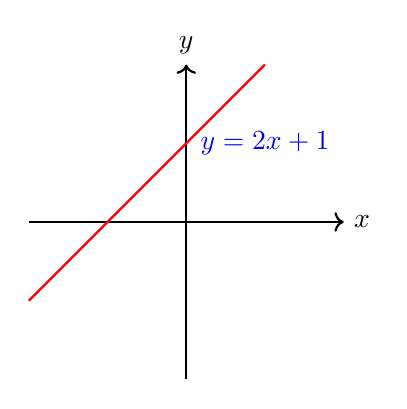
\begin{tikzpicture}[scale=1]
    % 绘制坐标轴
    \draw[->, thick] (-2,0) -- (2,0) node[right] {$x$};
    \draw[->, thick] (0,-2) -- (0,2) node[above] {$y$};
    % 绘制函数图像,添加 thick 选项使线条变粗
    \draw[domain=-2:1, smooth, variable=\x, red, thick] plot ({\x},{1*\x + 1});
    % 添加函数标签
    \node[blue] at (1,1) {$y = 2x + 1$};
\end{tikzpicture}
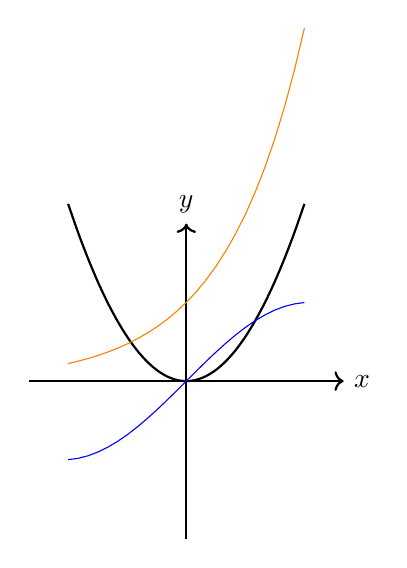
\begin{tikzpicture}[scale=1]
    % 绘制坐标轴
    \draw[->, thick] (-2,0) -- (2,0) node[right] {$x$};
    \draw[->, thick] (0,-2) -- (0,2) node[above] {$y$};
    % 绘制函数图像,添加 thick 选项使线条变粗
    \draw[domain=-1.5:1.5, smooth, variable=\x,  thick] plot ({\x},{\x*\x});
    % 添加函数标签
    \draw[domain=-1.5:1.5 ,color=blue] plot (\x,{sin(\x r)}); %r 表示弧度制

    \draw[domain=-1.5:1.5 ,color=orange] plot (\x,{exp(\x)}) ;
\end{tikzpicture}

\begin{tikzpicture}
    \draw (0,0) rectangle (4,4);
\end{tikzpicture}

\begin{tikzpicture}
    \draw (0,0) parabola (4,4);
  \end{tikzpicture}

  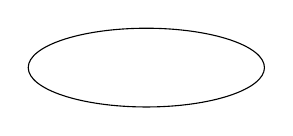
\begin{tikzpicture}
	\draw[scale=0.5] (0,0) ellipse (3cm and 1cm);
\end{tikzpicture}





    




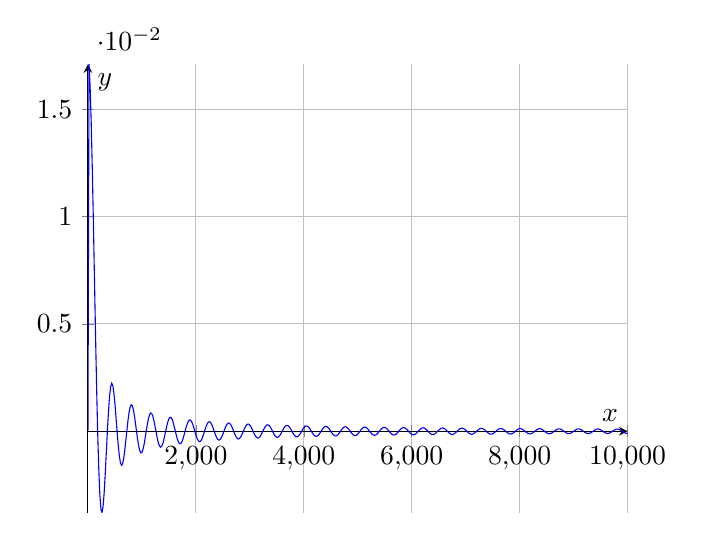
\begin{tikzpicture}
		\begin{axis}[
			axis lines =middle,
			xlabel = $x$,
			ylabel = {$y$},
			grid = major,
			]
			% 绘制函数 y = x^2
			\addplot [
			domain=0:10000, % 定义绘制区间
			samples=500, % 采样点数量,越高图像越平滑
			color=blue,
			]{(sin(x))/x };%基本上与数学环境中的函数差不多,去掉“\”就行了
		\end{axis}
	\end{tikzpicture}

\begin{tikzpicture}
		\begin{axis}[
			axis lines =middle,
			xlabel = $x$,
			ylabel = $y$,
			]
			\addplot [
			domain=-10:10, % 定义绘制区间
			samples=500, % 采样点数量,越高图像越平滑
			color=blue,
			]{(x*x) };%基本上与数学环境中的函数差不多,去掉“\”就行了
		\end{axis}
	\end{tikzpicture}

    \begin{tikzpicture}
        \begin{axis}[
            axis lines = middle,
            xlabel = $x$,
            ylabel = $y$,
            xmin = -2,
            xmax = 2,
            ymin = -2,
            ymax = 2,
            clip = false, % 设置不裁剪图形,也就是函数图像会超过坐标轴的范围
            axis line style={thick}, %使坐标轴变粗
            x axis line style={-Latex},
            y axis line style={-stealth},
            title = {取消刻度},   
            xtick=\empty,
            ytick=\empty %取消刻度
        ]
        \addplot [
            domain=-pi/2:pi/2 ,
            samples=500,
            color=blue
        ]{(sin(deg(x)))};
        \end{axis}
    \end{tikzpicture}

    \begin{tikzpicture}
        \begin{axis}[
            axis lines = middle, % 会影响x轴和y轴的相对位置
            xlabel = $x$,
            ylabel = $y$,
            xmin = -2,
            xmax = 2,
            ymin = -2,
            ymax = 2,
            clip = false, % 设置不裁剪图形,也就是函数图像会超过坐标轴的范围
            axis line style={thick}, %使坐标轴变粗
            x axis line style={-Latex},
            y axis line style={-stealth},
            title = {设置函数图像线宽:对数函数},   
            xtick=\empty,
            ytick=\empty %取消刻度
        ]
        \addplot [
            domain=0.1:pi/2 ,
            line width = 1.5pt,
            samples=500,
            % color=blue
        ]{(ln(x))};
        \end{axis}
    \end{tikzpicture}

    
\end{document}
